\documentclass[a4paper,11pt]{jsarticle}


% 数式
\usepackage{amsmath,amsfonts}
\usepackage{bm}
% 画像
\usepackage[dvipdfmx]{graphicx}
\bibliographystyle{myjunsrt}
\renewcommand{\bibname}{参考文献}


\begin{document}

\title{}
\author{}
\date{\today}
\maketitle

\section{tangent delta}

媒質に損失がある場合の電磁波に対する基本式は以下のようになる。

\begin{equation}
  \mathrm{rot}(\frac{1}{\mu(\boldsymbol{r})}\mathrm{rot}\boldsymbol{E}) = -\mu_0 \mathrm{rot}(\frac{\partial H}{\partial t})
\end{equation}
\begin{equation}
  \mathrm{rot}(\frac{\partial H}{\partial t}) = \epsilon(\boldsymbol{r})\epsilon_0 \frac{\partial^2 E}{\partial t^2} + \frac{\partial J}{\partial t}
\end{equation}


媒質に損失がある場合の特性値を考える。
ここで時間変動因子$exp(j\omega t)$ が入射することを考えると、そのときのマクスウェルの方程式は

\begin{equation} \label{eq:loss_electric_flux_density}
  \mathrm{rot} H = \epsilon \epsilon_0 \frac{\partial E}{\partial t} + \sigma \boldsymbol{E} = (j\omega\epsilon\epsilon_0 + \sigma)\boldsymbol{E}
\end{equation}

と書くことができる。このとき、
式\ref{eq:loss_electric_flux_density}の右辺が電束密度$\boldsymbol{D}$から生じているとみなし、

\begin{equation} \label{eq:electric_flux_density}
  \boldsymbol{D} = C\epsilon \epsilon_0 \boldsymbol{E}(\boldsymbol{r})exp(j\omega t)
\end{equation}

として代入しなおすと、$C=1 - j\sigma / \omega\epsilon\epsilon_0$を得る。
これで電束密度は

\begin{equation} \label{eq:electric_flux_density_tangent_delta}
  \boldsymbol{D} = \dot{\epsilon} \epsilon_0 \boldsymbol{E} = \epsilon \epsilon_0 (1 - j\tan\delta)\boldsymbol{E}
\end{equation}

\begin{equation} \label{eq:epsilon_dot}
  \dot{\epsilon} = \epsilon (1 - j\tan\delta)
\end{equation}

\begin{equation} \label{eq:tangent_delta}
  \tan \delta = \frac{\sigma}{\omega\epsilon\epsilon_0}
\end{equation}

とあらわすことができる。
式\ref{eq:tangent_delta}はタンデルタと呼ばれ、伝導電流と変位電流の比を表す。
$\delta$を損失角という。高周波では、$\dot{\epsilon}$の実部の寄与が大きくなり、低周波では虚部の寄与が大きくなる。
言い換えると、誘電体に交流電場が加わったときにそのエネルギーの一部が熱となってしまう比率ともいえる。

\section{表皮効果}

本研究における実験では銅板でミリ波を遮断することが多くある。
導体である銅板の導電率$\sigma$は非常に大きくなり、
振幅減衰定数$\alpha$と位相定数$\beta$は

\begin{equation}
  \alpha \approx \beta \approx \sqrt[]{\frac{\omega\mu\mu_0\sigma}{2}}
\end{equation}

のように同じ値に近似できる。
つまり、導電率$\sigma$の増加とともに電磁波の減衰が大きなることを示し、
電磁波は指数関数的に減衰する。
入社電磁波の振幅が表面での値に対して$1/e$になるときの深さ$\delta$を
表皮深さと呼び、次の式で表すことができる。

\begin{equation}
  \delta = \frac{1}{\alpha} = \sqrt[]{\frac{2}{\omega\mu\mu_0\sigma}}
\end{equation}

このことから、電磁波の周波数が上昇し、導電率が大きくなるほど表皮深さが浅くなることを示す。
このとき、銅板の表面近傍にのみ電流が流れ、表皮効果(skin effect)と呼ぶ。
電流が流れるということは抵抗が存在することを意味し、表皮抵抗は

\begin{equation}
  Re\{Z_W\} = \sqrt[]{\frac{\omega\mu\mu_0}{2}} = \frac{1}{\delta\sigma}
\end{equation}

とあらわされる。
ミリ波を遮断するために銅板を使うのは相性がいいといえる。

\section{Snellの法則}

異なる媒質の境界面では、電磁波の反射や屈折が起こる。
これはSnellの法則によって記述され、本研究における重要な法則になる。
こちらはマクスウェルの方程式と境界条件を用いて導き出すことができる。

媒質の境界面をx-y平面、各領域内で媒質がy方向に一様とする。
比誘電率と比透磁率を第一媒質に対して$\dot{\epsilon_1}$、$\mu_1$、
第二媒質に対して$\dot{\epsilon_2}$、$\mu_2$とする。
損失があるときの複素比誘電率を、次のようにおく。
$i$はそれぞれの媒質を表すので、1と2の値をとる。

\begin{equation}
  \dot{\epsilon_i} = \epsilon_i(1 - j\frac{\sigma_i}{\omega\epsilon_i\epsilon_0})
\end{equation}

ただし、$\sigma$は導電率、$\omega$は電磁波の角周波数、$\epsilon$は無損失時の比誘電率、
$\epsilon_0$は真空の誘電率を表す。
今回の比透磁率$\mu$は実数とする。
ここで各媒質の波数の大きさは$k$として以下のようになる。
$c$は真空中の光速である。

\begin{equation}
  k_i = \frac{\omega\sqrt[]{\dot{\epsilon_i}\mu_i}}{c}
\end{equation}

ここでTE波を例にSnellの法則を導き出す。
TE波は電界の振動方向が紙面に垂直であり、伝搬方向に電界成分を持たない。
紙面に垂直な方向は$y$軸なので、その電界を$E^i_y$として

\begin{equation}
  E^i_y = A_{iS}\exp[j(\omega t - \boldsymbol{k}_i\cdot\boldsymbol{r})]
\end{equation}

と書く。$A_{iS}$は電界振幅、$\boldsymbol{k}_i$は媒質中の波数ベクトル、
$\boldsymbol{r}$は波面の任意の点への位置ベクトルとなる。
添え字の$i$は3つの状態を持ち、入射・透過・反射をそれぞれ$i$、$t$、$r$で表す。

\section{全反射}

電磁波が密な媒質から疎な媒質に入射する場合、
入射角を徐々に大きくすると入射角より屈折角のほうが先に90度となる。
このとき、入射電磁波が透過することなく境界面で反射後に
すべて入射側に戻る現象を全反射という。

全反射時のTE波の透過電界成分は以下のように書ける。

\begin{equation}
  E^t_y = \exp[-j(\sqrt[]{\epsilon_1\mu_1}k_0\sin\theta_t)x]\exp\left(-\frac{z}{z_g}\right)
\end{equation}

\begin{equation}
  z_g = \frac{c}{\omega\sqrt[]{\epsilon_1\mu_1\sin^{2}\theta - \epsilon_2\mu_2}}
\end{equation}

$z_g$ は第二媒質への電界の侵入深さを表し、電磁波は境界面へわずかにしみでていることがわかる。
全反射時にも電磁波は境界面の反対側にもわずかに浸みだす。
この成分をevanescent波と呼ぶ。
電磁界の浸みこみと合わせて、反射点もずれる。
このずれのことをグースヘンヒェンシフトと呼ぶ。
誘電体導波路、光ファイバーを利用する際に重要となる。

電磁波は境界面の反対側にもわずかに浸みだすが、
注意しなければならないのはエネルギーは浸みださないことである。
振幅反射係数の和はすべて$1$となり、エネルギーもすべて反射する。

\begin{figure}
  \begin{center}
    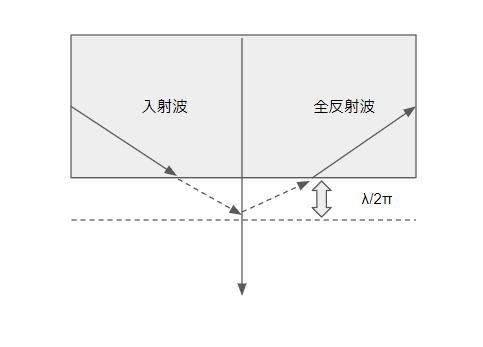
\includegraphics[clip, keepaspectratio, width=0.5\linewidth]{img/insertion_reflection_evanescence.png}
    \caption{evanescent成分の浸みだし}
    \label{fig:insertion_reflection_evanescent}
  \end{center}
\end{figure}


\section{電波の伝搬ロス}

自由空間を伝搬する電波の損失$L$は以下の式で表される。

\begin{equation}
  L = \left(\frac{4\pi d}{\lambda} \right)^2
\end{equation}

このとき$\lambda$は波長、$d$は距離となる。
例えば28GHzの電波を考えると波長は10mmなので、
0.25cm離れたところでは-49.3dBの減衰がみられる。
800MHz(波長375mm)の電波であれば、
同じ-49.3dBの減衰がみられるのは10m離れたところとなる。

TODO:画像追加

\section{リンクバジェット}

\section{曲がるアンテナ}

先行研究として株式会社NTTドコモが開発した曲がるアンテナが存在する
\cite{bending_antenna}。

\newpage
\addcontentsline{toc}{chapter}{\bibname}
\bibliography{common_bibliography}

\end{document}